\documentclass{beamer}
\usepackage{amsmath}
\usepackage{hyperref}
\usepackage{listings}
\usepackage{xcolor}
\hypersetup{colorlinks=true, citecolor=blue, filecolor=blue, linkcolor=blue, urlcolor=blue}
\definecolor{codegreen}{rgb}{0,0.6,0}
\definecolor{codegray}{rgb}{0.5,0.5,0.5}
\definecolor{codepurple}{rgb}{0.58,0,0.82}
\definecolor{backcolour}{rgb}{0.95,0.95,0.92}
 
\lstdefinestyle{mystyle}{
    backgroundcolor=\color{backcolour},   
    commentstyle=\color{codegreen},
    keywordstyle=\color{magenta},
    numberstyle=\tiny\color{codegray},
    stringstyle=\color{codepurple},
    basicstyle=\ttfamily\footnotesize,
    breakatwhitespace=false,         
    breaklines=true,                 
    captionpos=b,                    
    keepspaces=true,                 
    %numbers=left,                    
    numbersep=5pt,                  
    showspaces=false,                
    showstringspaces=false,
    showtabs=false,                  
    tabsize=2
}
 
\lstset{style=mystyle}

\mode<presentation> {

% The Beamer class comes with a number of default slide themes
% which change the colors and layouts of slides. Below this is a list
% of all the themes, uncomment each in turn to see what they look like.

%\usetheme{default}
\usetheme{AnnArbor}
%\usetheme{Antibes}
%\usetheme{Bergen}
%\usetheme{Berkeley}
%\usetheme{Berlin}
%\usetheme{Boadilla}
%\usetheme{CambridgeUS}
%\usetheme{Copenhagen}
%\usetheme{Darmstadt}
%\usetheme{Dresden}
%\usetheme{Frankfurt}
%\usetheme{Goettingen}
%\usetheme{Hannover}
%\usetheme{Ilmenau}
%\usetheme{JuanLesPins}
%\usetheme{Luebeck}
%\usetheme{Madrid}
%\usetheme{Malmoe}
%\usetheme{Marburg}
%\usetheme{Montpellier}
%\usetheme{PaloAlto}
%\usetheme{Pittsburgh}
%\usetheme{Rochester}
%\usetheme{Singapore}
%\usetheme{Szeged}
%\usetheme{Warsaw}

% As well as themes, the Beamer class has a number of color themes
% for any slide theme. Uncomment each of these in turn to see how it
% changes the colors of your current slide theme.

%\usecolortheme{albatross}
%\usecolortheme{beaver}
%\usecolortheme{beetle}
%\usecolortheme{crane}
%\usecolortheme{dolphin}
%\usecolortheme{dove}
%\usecolortheme{fly}
%\usecolortheme{lily}
%\usecolortheme{orchid}
%\usecolortheme{rose}
%\usecolortheme{seagull}
%\usecolortheme{seahorse}
%\usecolortheme{whale}
%\usecolortheme{wolverine}

%\setbeamertemplate{footline} % To remove the footer line in all slides uncomment this line
\setbeamertemplate{footline}[page number] % To replace the footer line in all slides with a simple slide count uncomment this line

\setbeamertemplate{navigation symbols}{} % To remove the navigation symbols from the bottom of all slides uncomment this line
}

\usepackage{graphicx} % Allows including images
\usepackage{booktabs} % Allows the use of \toprule, \midrule and \bottomrule in tables
%\usepackage {tikz}
\usepackage{tkz-graph}
\GraphInit[vstyle = Shade]
\tikzset{
  LabelStyle/.style = { rectangle, rounded corners, draw,
                        minimum width = 2em, fill = yellow!50,
                        text = red, font = \bfseries },
  VertexStyle/.append style = { inner sep=5pt,
                                font = \normalsize\bfseries},
  EdgeStyle/.append style = {->, bend left} }
\usetikzlibrary {positioning}
%\usepackage {xcolor}
\definecolor {processblue}{cmyk}{0.96,0,0,0}
%----------------------------------------------------------------------------------------
%	TITLE PAGE
%----------------------------------------------------------------------------------------

\title[Uncertainty]{Numerical Optimization 17: Uncertainty} %

\author{Qiang Zhu} % Your name
\institute[University of Nevada Las Vegas] % Your institution as it will appear on the bottom of every slide, may be shorthand to save space
{
University of Nevada Las Vegas\\ % Your institution for the title page
\medskip
}
\date{\today} % Date, can be changed to a custom date

\begin{document}

\begin{frame}
\titlepage % Print the title page as the first slide
\end{frame}

\begin{frame}
\frametitle{Overview} % Table of contents slide, comment this block out to remove it
\tableofcontents % Throughout your presentation, if you choose to use \section{} and \subsection{} commands, these will automatically be printed on this slide as an overview of your presentation
\end{frame}

%----------------------------------------------------------------------------------------
%	PRESENTATION SLIDES
%----------------------------------------------------------------------------------------

%------------------------------------------------

\section{Uncertainty}
\begin{frame}{Uncertainty}
In many engineering tasks, however, there may be uncertainty due to a number of factors, such as model approximations, imprecision, and fluctuations of parameters over time. We want to minimize $f(x, z)$, but we do not have control over $z$. Feasibility depends on both the design vector $x$ and the uncertain vector $z$. 
\begin{figure}
\centering
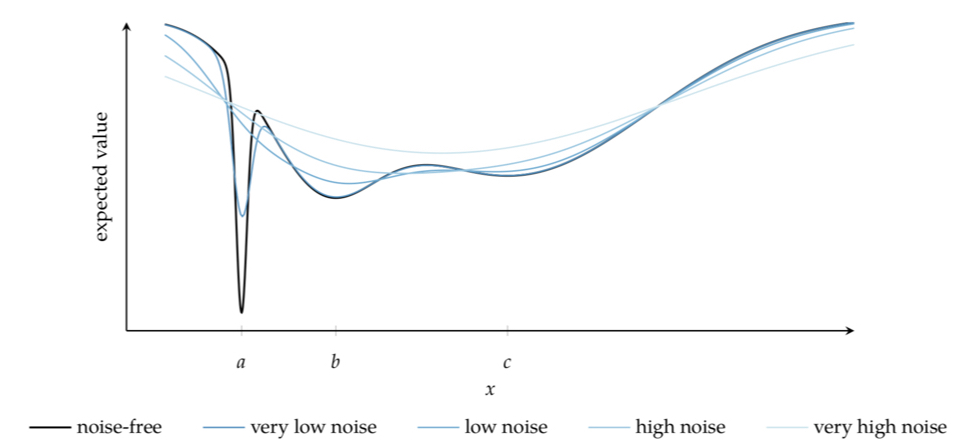
\includegraphics[width=110mm]{Figs/uncertainty.jpeg}
\end{figure} 
\end{frame}

\section{Polynomial Chaos}
\begin{frame}{Polynomial chaos}
\textcolor{blue}{Polynomial chaos} is a method for fitting a polynomial to $f(x, z)$ and using the resulting surrogate model to estimate the mean and variance. 

In one dimension, we approximate $f(z)$ with a surrogate model consisting of $k$ polynomial basis functions, $b_1, \cdots, b_k$:
\begin{equation*}
    f(z) = \hat{f}(z) = \sum_{i=1}^k \theta_i b_i(z)
\end{equation*}
The mean of $\hat{f}$ can be derived as follows
\begin{equation*}
\begin{split}
    \hat{\mu} & = \int_Z p(z)\hat{f}(z) dz = \int_Z \sum_{i=1}^k p(z) \theta_i b_i(z) dx
    = \sum_{i=1}^k \int_Z \theta_i b_i(z) p(z)dz \\
              & = \theta_1 \int_Z b_1(z) p(z)dz + \cdots + \theta_n \int_Z b_n(z) p(z)dz
\end{split}
\end{equation*}
\end{frame}

\begin{frame}{Polynomial chaos}
The variance of $\hat{f}$ can be derived as follows
\begin{equation*}
\begin{split}
    \hat{\sigma} & = \mathbb{E}[\hat{f}^2] - (\mathbb{E}[\hat{f}])^2
    = \int_Z p^2(z)\hat{f}(z) dz - \mu^2\\
    &= \int_Z \sum_{i=1}^k\sum_{j=1}^k  \theta_i\theta_j b_i(z)b_j(z)p(z)dz - \mu^2\\
    & = \int_Z \bigg( \sum_{i=1}^k \theta_i^2 b_i^2(z) + 2\sum_{i=2}^k\sum_{j=1}^{i-1} \theta_i\theta_j b_i(z)b_j(z)\bigg)p(z)dz -\mu^2 \\
    & =  \sum_{i=1}^k \theta_i^2 \int_Z b_i^2(z)dz + 2\sum_{i=2}^k\sum_{j=1}^{i-1} \theta_i\theta_j \int_Z b_i(z)b_j(z)p(z)dz
    - \mu^2
\end{split}
\end{equation*}
\end{frame}

\section{Orthogonal polynomial basis}
\begin{frame}{Orthogonal polynomial basis}
The mean and variance can be efficiently computed if the basis functions are chosen to be orthogonal under $p$. Two basis functions $b_i$ and $b_j$ are orthogonal with respect to a probability density $p(z)$ if
\begin{equation*}
     \int_Z b_i(z)b_j(z)p(z)dz = 0. ~({\textrm{if~}} i\neq j)
\end{equation*}

If the chosen basis functions are all orthogonal to one another and the first basis function is $b_1(z) = 1$, the mean is:
\begin{equation*}
\begin{split}
    \hat{\mu} & = \theta_1 \int_Z b_1(z) p(z)dz + \cdots + \theta_n \int_Z b_n(z) p(z)dz\\
    & = \theta_1 \int_Z b^2_1(z) p(z)dz + \cdots + \theta_n \int_Z b_1(z) b_n(z) p(z)dz\\
    & = \theta_1
\end{split}
\end{equation*}

\end{frame}

\begin{frame}{Orthogonal polynomial basis}
Similarly, the variance is 
\begin{equation*}
\begin{split}
    \hat{\sigma} & = \sum_{i=1}^k \theta_i^2 \int_Z b_i^2(z)dz + 2\sum_{i=2}^k\sum_{j=1}^{i-1} \theta_i\theta_j \int_Z b_i(z)b_j(z)p(z)dz - \mu^2\\
    & = \sum_{i=1}^k \theta_i^2 \int_Z b_i^2(z)dz - \mu^2 \\
    & = \theta_1^2 \int_Z b_1^2(z)dz - \sum_{i=1}^k \theta_i^2 \int_Z b_i^2(z)dz- \mu^2 \\
    & = \sum_{i=1}^k \theta_i^2 \int_Z b_i^2(z)dz
\end{split}
\end{equation*}

\end{frame}

\begin{frame}{Orthogonal polynomial basis}
The mean thus falls immediately from fitting a surrogate model to the observed data, and the variance can be very efficiently computed given the values $\int_Z b_i^2(z)p(z)dz$ for a choice of basis functions and probability distribution. All orthogonal polynomials satisfy the recurrence relation:
\begin{equation*}
    b_{i+1}(z) = 
    \begin{cases}
    (z-a_i)b_i(z) & i=1\\
    (z-a_i)b_i(z) - \beta_i b_{i-1}z & {\textrm{else}}
    \end{cases}
\end{equation*}
with $b_1(z)$ = 1 and weights
\begin{equation*}
    \begin{split}
    \alpha_i &= \frac{\int_Z z b_i^2(z)p(z)dz} {\int_Z b_i^2(z)p(z)dz}\\
    \beta_i &= \frac{\int_Z b_i^2(z)p(z)dz}{\int_Z b_{i-1}^2(z)p(z)dz}      
    \end{split}
\end{equation*}
The recurrence relation can be used to generate the basis functions. Each basis function $b_i$ is a polynomial of degree $i-1$. 

\end{frame}

\begin{frame}{Orthogonal polynomial basis functions}
\begin{figure}
\centering
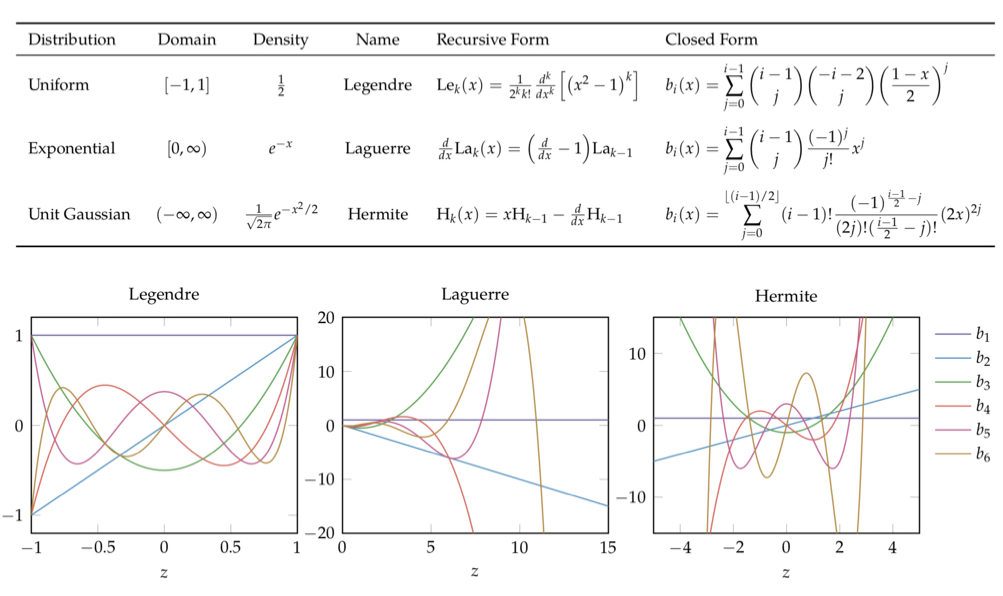
\includegraphics[width=120mm]{Figs/orthogonal.jpeg}
\end{figure} 
\end{frame}

\section{Coefficients}
\begin{frame}{Coefficients}
The coefficients $\theta_1, \cdots, \theta_k$ can be inferred by exploiting the orthogonality of the basis functions, producing an integration term amenable to \textcolor{blue}{Gaussian quadrature}.
\begin{equation*}
\begin{split}
    f(z) &= \sum_{i=1}^k \theta_i b_i(z)\\
    \int_Z f(z)b_j(z)p(z)dz &= \int_Z \bigg(\sum_{i=1}^k \theta_i b_i(z) \bigg) b_j(z)p(z)dz\\
    &= \sum_{i=1}^k \theta_i \int_Z b_i(z)b_j(z)p(z)dz \\
    &= \theta_j \int_Z b_j(z)p(z)dz\\
    \implies \theta_j &= \frac{\int_Z f(z)b_j(z)p(z)dz}{\int_Z b_j(z)p(z)dz}
\end{split}
\end{equation*}
\end{frame}

\section{Multivariate}
\begin{frame}{Multivariate}
Polynomial chaos can be applied to functions with multiple random inputs. Multivariate basis functions over m variables are constructed as a product over univariate orthogonal polynomials:
%\begin{equation*}
%\begin{split}
%\end{split}
%\end{equation*}
\end{frame}

\section{Summary}
\begin{frame}{Summary}
    \begin{itemize}
        \item Polynomial chaos is a powerful uncertainty propagation technique basedon orthogonal polynomials.
        \item Bayesian Monte Carlo uses Gaussian processes to efficiently arrive at the moments with analytic results for Gaussian kernels.
    \end{itemize}
\end{frame}
\end{document}

